%%% LaTeX Template: Two column article
%%%
%%% Source: http://www.howtotex.com/
%%% Feel free to distribute this template, but please keep to referal to http://www.howtotex.com/ here.
%%% Date: February 2011

%%% Preamble
\documentclass[	DIV=calc,%
							paper=a4,%
							fontsize=12pt,%
							onecolumn]{scrartcl}	 					% KOMA-article class

\usepackage{lipsum}													% Package to create dummy text
\usepackage[brazil]{babel}										% English language/hyphenation
\usepackage[protrusion=true,expansion=true]{microtype}				% Better typography
\usepackage{amsmath,amsfonts,amsthm}					% Math packages
\usepackage[pdftex]{graphicx}									% Enable pdflatex
\usepackage[svgnames]{xcolor}									% Enabling colors by their 'svgnames'
\usepackage[hang, small,labelfont=bf,up,textfont=it,up]{caption}	% Custom captions under/above floats
\usepackage{epstopdf}												% Converts .eps to .pdf
\usepackage{subfig}													% Subfigures
\usepackage{booktabs}												% Nicer tables
\usepackage{fix-cm}													% Custom fontsizes
\usepackage[utf8]{inputenc}
\usepackage[top=2.5cm, bottom=2.5cm, left=2.5cm, right=2.5cm]{geometry}
\usepackage[ddmmyyyy]{datetime}
\addto\captionsenglish{%
	\renewcommand\tablename{Tabela}
	\renewcommand\figurename{Figura}
} 
 

 
%%% Custom sectioning (sectsty package)
\usepackage{sectsty}													% Custom sectioning (see below)
\allsectionsfont{%															% Change font of al section commands
	\usefont{OT1}{phv}{b}{n}%										% bch-b-n: CharterBT-Bold font
	}

\sectionfont{%																% Change font of \section command
	\usefont{OT1}{phv}{b}{n}%										% bch-b-n: CharterBT-Bold font
	}



%%% Headers and footers
\usepackage{fancyhdr}												% Needed to define custom headers/footers
	\pagestyle{fancy}														% Enabling the custom headers/footers
\usepackage{lastpage}	

% Header (empty)
\lhead{}
\chead{}
\rhead{}
% Footer (you may change this to your own needs)

%% ====================================
%% ====================================
%% mude o rodape  do projeto
%% ====================================
%% ====================================

\lfoot{\footnotesize \texttt{Cabeamento estruturado} \textbullet ~UBS}


\cfoot{}
\rfoot{\footnotesize página \thepage\ de \pageref{LastPage}}	% "Page 1 of 2"
\renewcommand{\headrulewidth}{0.0pt}
\renewcommand{\footrulewidth}{0.4pt}



%%% Creating an initial of the very first character of the content
\usepackage{lettrine}
\newcommand{\initial}[1]{%
     \lettrine[lines=3,lhang=0.3,nindent=0em]{
     				\color{DarkGoldenrod}
     				{\textsf{#1}}}{}}



%%% Title, author and date metadata
\usepackage{titling}															% For custom titles

\newcommand{\HorRule}{\color{DarkGoldenrod}%			% Creating a horizontal rule
									  	\rule{\linewidth}{1pt}%
										}

\pretitle{\vspace{-30pt} \begin{flushleft} \HorRule 
				\fontsize{50}{50} \usefont{OT1}{phv}{b}{n} \color{DarkRed} \selectfont 
				}

%% ====================================
%% ====================================
%% mude o titulo  do projeto
%% ====================================
%% ====================================

\title{Projeto de Cabeamento Estruturado Para Unidade Básica de Saúde - UBS }					% Title of your article goes here

%% ====================================



\posttitle{\par\end{flushleft}\vskip 0.5em}

\preauthor{\begin{flushleft}
					\large \lineskip 0.5em \usefont{OT1}{phv}{b}{sl} \color{DarkRed}}
\author{Marcelo Rodrigo Schmidt, Maicon Fernando de Oliveira }  	% Author name goes here


\postauthor{\footnotesize \usefont{OT1}{phv}{m}{sl} \color{Black} 
					\\Universidade Tecnológica Federal do Paraná - Câmpus Cornélio Procópio 								% Institution of author
					\par\end{flushleft}\HorRule}

\date{}																				% No date




%%% Begin document
\begin{document}
\maketitle
\thispagestyle{fancy} 	
\thispagestyle{empty}		% Enabling the custom headers/footers for the first page 
% The first character should be within \initial{}




%% ====================================
%% ====================================
%% mude o resumo  do projeto
%% ====================================
%% ====================================
\initial{E}\textbf{ste projeto tem como propósito a estruturação de cabos e equipamentos da nova Unidade Básica de Saúde (UBS) do município de Pato Bragado, como trata-se de um novo prédio da Secretaria Municipal de Saúde, não existe nenhuma estrutura de rede. Neste projeto serão apresentadas as plantas físicas do prédio e do rack de rede; a elaboração da planta lógica; todos os equipamentos de rede que serão utilizados e o levantamento de quantidade/custo total do projeto. Dentre as atividades que serão executadas estarão: Montagem e organização do rack de piso para acomodação dos equipamentos e cabos; instalação de cabos de rede nas salas para uso dos equipamentos e instalação dos próprios equipamentos que utilizarão a rede.}

%% ====================================
\begin{figure}
	\centering
	
\includegraphics{utfpr}
\end{figure}

\vspace{2cm}
\centerline{\textit{\textbf{\today}}}

\clearpage
    \renewcommand*\listfigurename{Lista de figuras}
\listoffigures


\clearpage
\renewcommand{\contentsname}{Sumário}
\tableofcontents
\clearpage

%% ====================================
%% ====================================
%% Inicio do texto
%% ====================================
%% ====================================
\section{Introdução}
A Unidade Básica de Saúde(UBS) foi construída recentemente, então, no momento não existe nenhuma instalação de rede no local. 
Esse projeto visa estruturar essa UBS com rack de rede e demais equipamentos passivos e ativos de categoria 6.
Ao final da estruturação a rede deverá ser utilizada por aproximadamente 20 computadores; 5 impressoras de rede e um cartão-ponto localizados nas diversas salas do prédio. Uma expansão futura é possível até número máximo de 41 dispositivos sem precisar acrescentar nada a estrutura, ultrapassando este número será necessário a compra de mais equipamentos como switch; conectores etc.

\subsection{Benefícios}
Existem vários outros lugares com estruturas já montadas na Prefeitura de Pato Bragado que não contaram com um projeto em seu início, ocasionando vários problemas de rede, portanto, o principal benefício desse projeto será evitar tais problemas e criar um rede organizada e estruturada de categoria 6. Sendo uma rede gigabit e toda estruturada, comportará muito bem todos os equipamentos e sistemas que serão utilizados, agilizando assim o atendimento da UBS.

\subsection{Organizações Envolvidas}
Para tal implantação do cabeamento estruturado será necessário o envolvimento da empresa terceirizada que detém contrato de link de internet e Vlan por fibra óptica que realizará a instalação da mesma na sala onde ficarão alojados todos os equipamentos de rede.
Para todo o restante, desde montagem de rack, lançamento dos cabos, crimpagem e demais instalações e configurações estarão envolvidos os três coloboradores que trabalham no Departamento de Tecnologias e Sistemas de Informação da Prefeitura Municipal. Os mesmos serão responsáveis no futuro pela manutenção da rede neste local. 

%\section{Estado atual}
%Aprente o estado atual da rede. Caso não %tenha rede, desconsiderar esta seção.

%Caso tenha rede, deixe claro:
%\begin{itemize}
%	\item os passivos de rede atuais:path panels, cabos, etc..;
%	\item as principais reclamações dos usuários. Qual o principal motivo da reestruturação? Efetue uma pesquisa junto aos colaboradores para determinar quais problemas a rede apresenta.
%	\item Observações. Analise a rede e verifique se há estruturas que não se enquadram nas normas ou que indicam suspeita de problemas.
%\end{itemize}

\section{Requisitos}
\begin{itemize}
\item Todos os equipamentos deverão ser de padrão Gigabit Cat6.
\item Deverá ter um rack de piso para acomodar todos os equipamentos necessários e a entrada dos cabos de rede.
\item Deverá ter um nobreak com autonomia de 4 horas para atender todos os equipamentos instalados no rack.
\item O rack com todos os equipamentos e cabeamento deverão ficar em uma sala refrigerado com ar condicionado separada de todas as demais.	
\end{itemize}

\section{Usuários e Aplicativos}
 
\subsection{Usuários}
Serão aproximadamente vinte usuários, que utilizarão na rede equipamentos como: computadores; notebooks; impressoras e cartão-ponto.

\subsection{Aplicativos}
Os aplicativos que serão utilizados com maior frequência são: O sistema geral de atendimento da Unidade Básica de Saúde que necessita um quantidade mínima de velocidade de internet para perfeito funcionamento (sistema web). Já o cartão ponto, o sistema de compras e as impressoras necessitam apenas de rede para seu funcionamento.

\section{Estrutura predial existente}
O prédio é novo e recentemente construído, em seu projeto já foi previsto a rede lógica, deste modo, em todas as salas já estão instaladas caixas embutidas nas paredes interligadas com eletro dutos até na sala central onde ficará o rack. Nesta, os eletrodutos descem por um buraco na lage. Os pontos de rede irão variar a distância de 8 até 40 metros. A estrutura básica já está pronta faltando apenas a montagem e instalação dos equipamentos e cabos. Todos os pontos serão interligados do patch panel ao seu respectivo mutoa/wallplate, sendo utilizados patch cords para ligação entre patch panel e switch e entre wallplate/mutoa e dispositivos. 

\section{Planta Lógica - Elementos estruturados}

\subsection{Estado atual}
Segue abaixo planta baixa da UBS (Unidade Básica de Saúde) que encontra-se recentemente construída e com todos os eletrodutos prontos para lançamento dos cabos e instalação dos esquipamentos. 
 
\begin{figure}
	\centering
	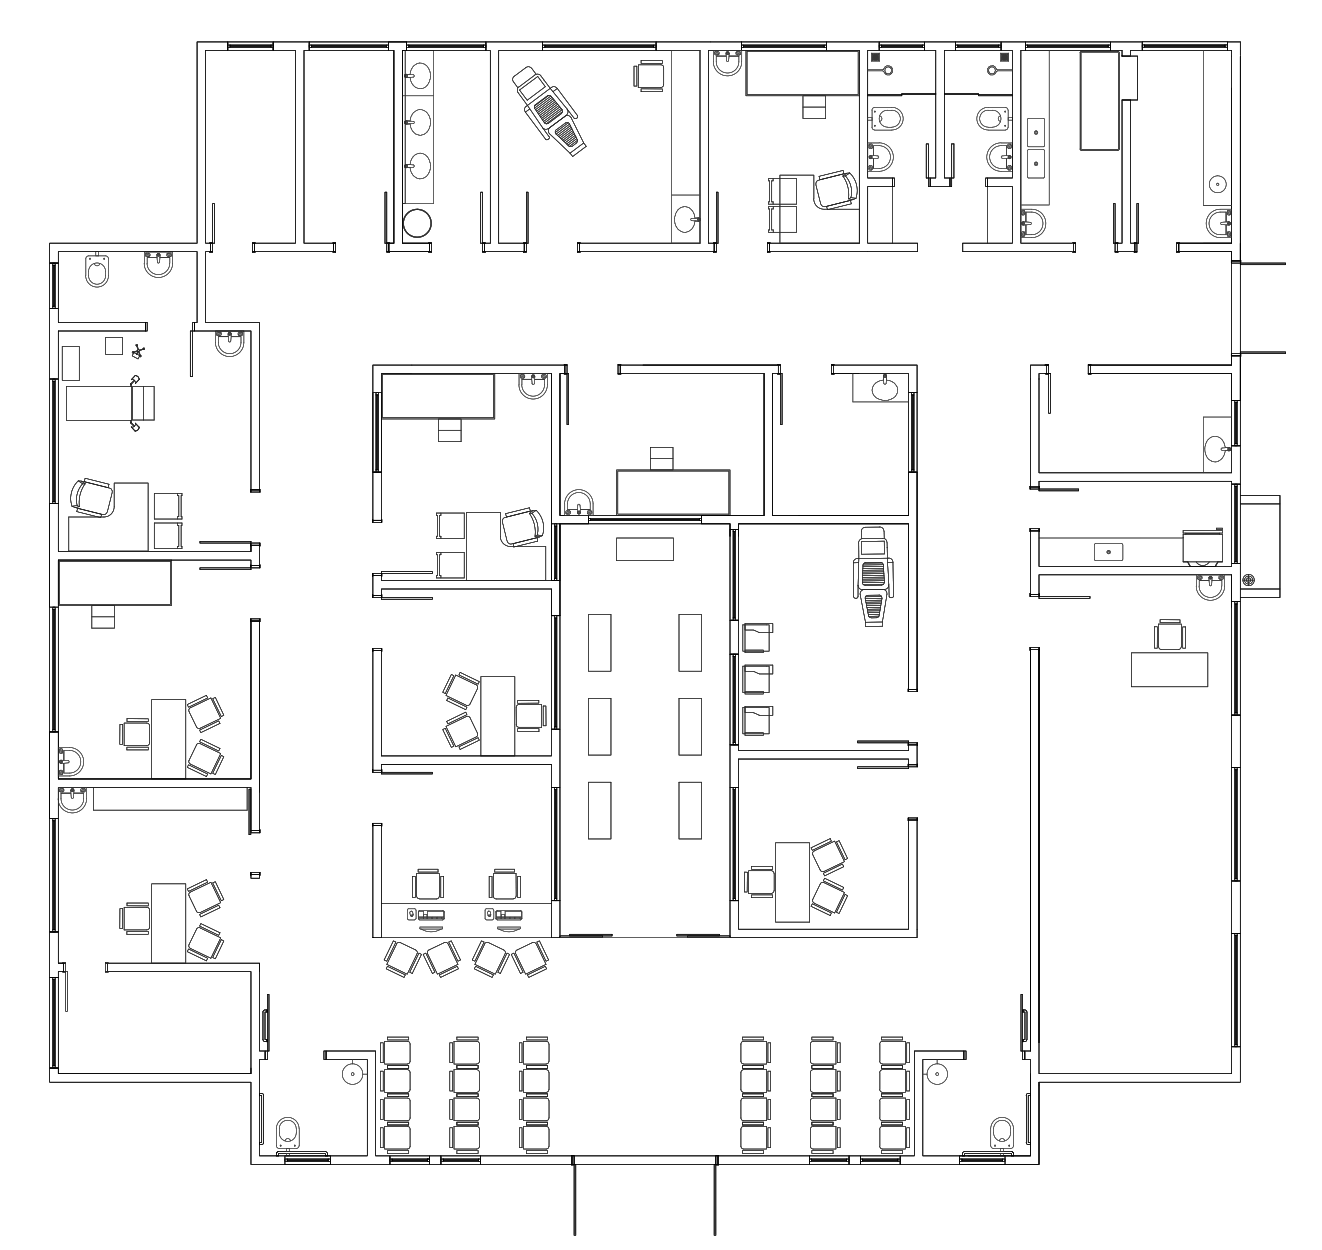
\includegraphics[width=\textwidth]{fig1}
	\caption{Planta baixa da UBS}
	\label{fig1}
\end{figure}

\begin{figure}
	\centering
	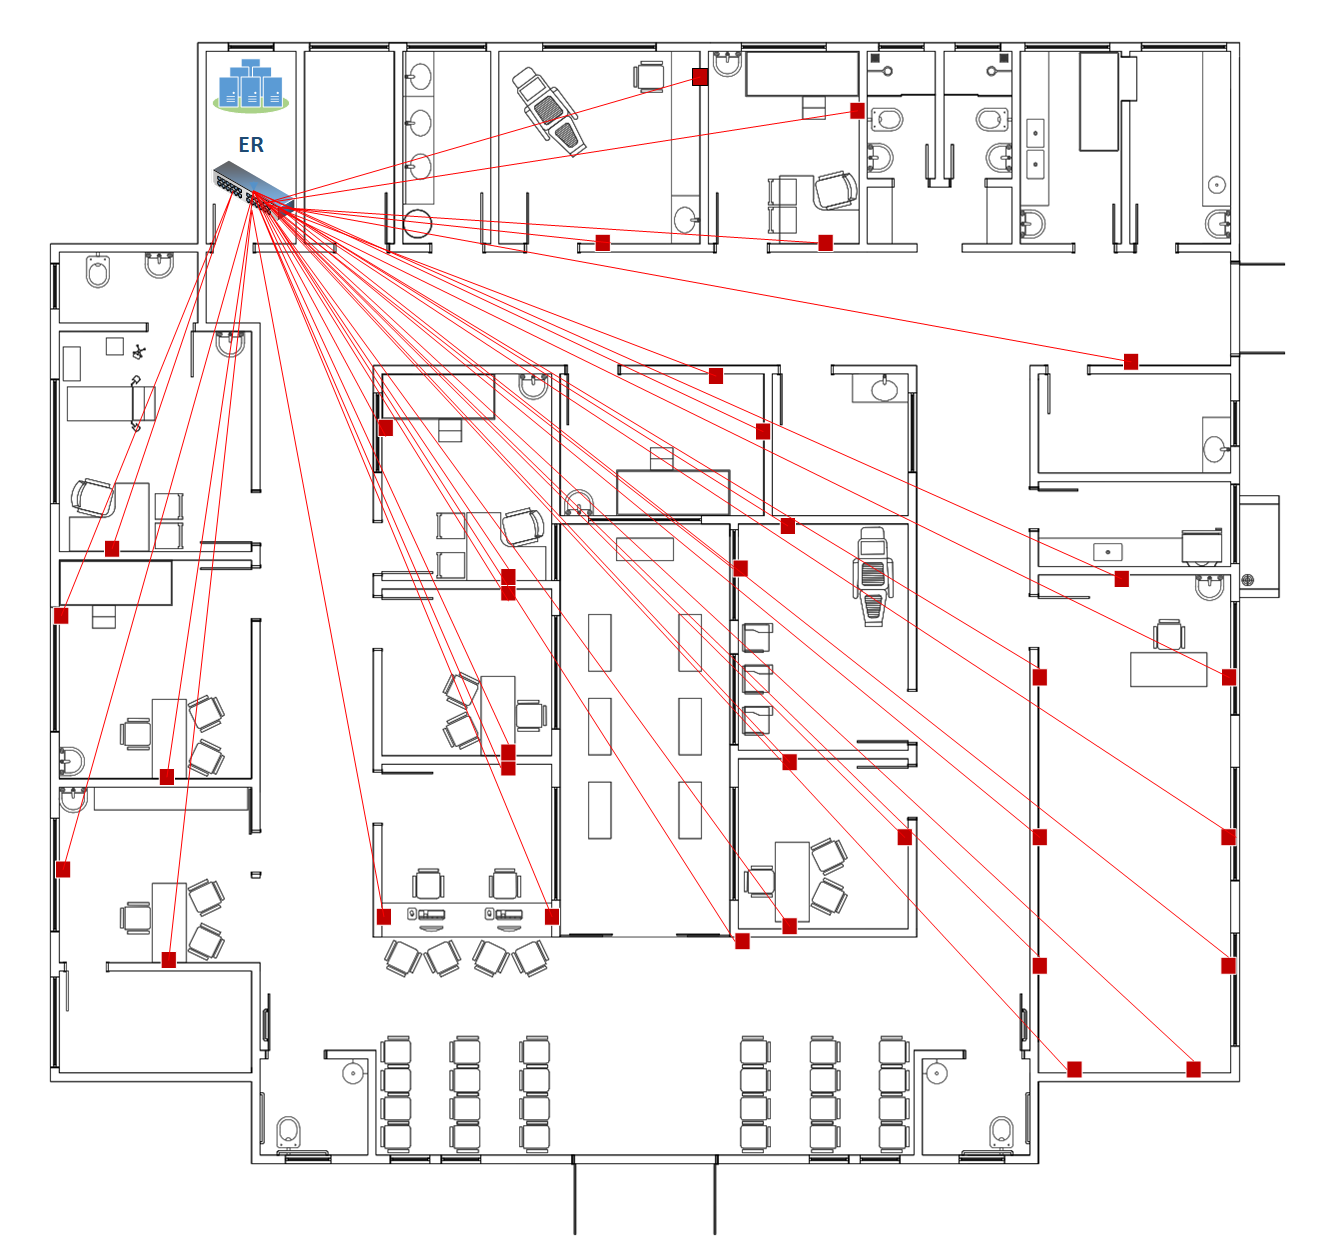
\includegraphics[width=\textwidth]{fig2}
	\caption{Cabeamento e pontos de rede}
	\label{fig2}
\end{figure}

\begin{figure}
	\centering
	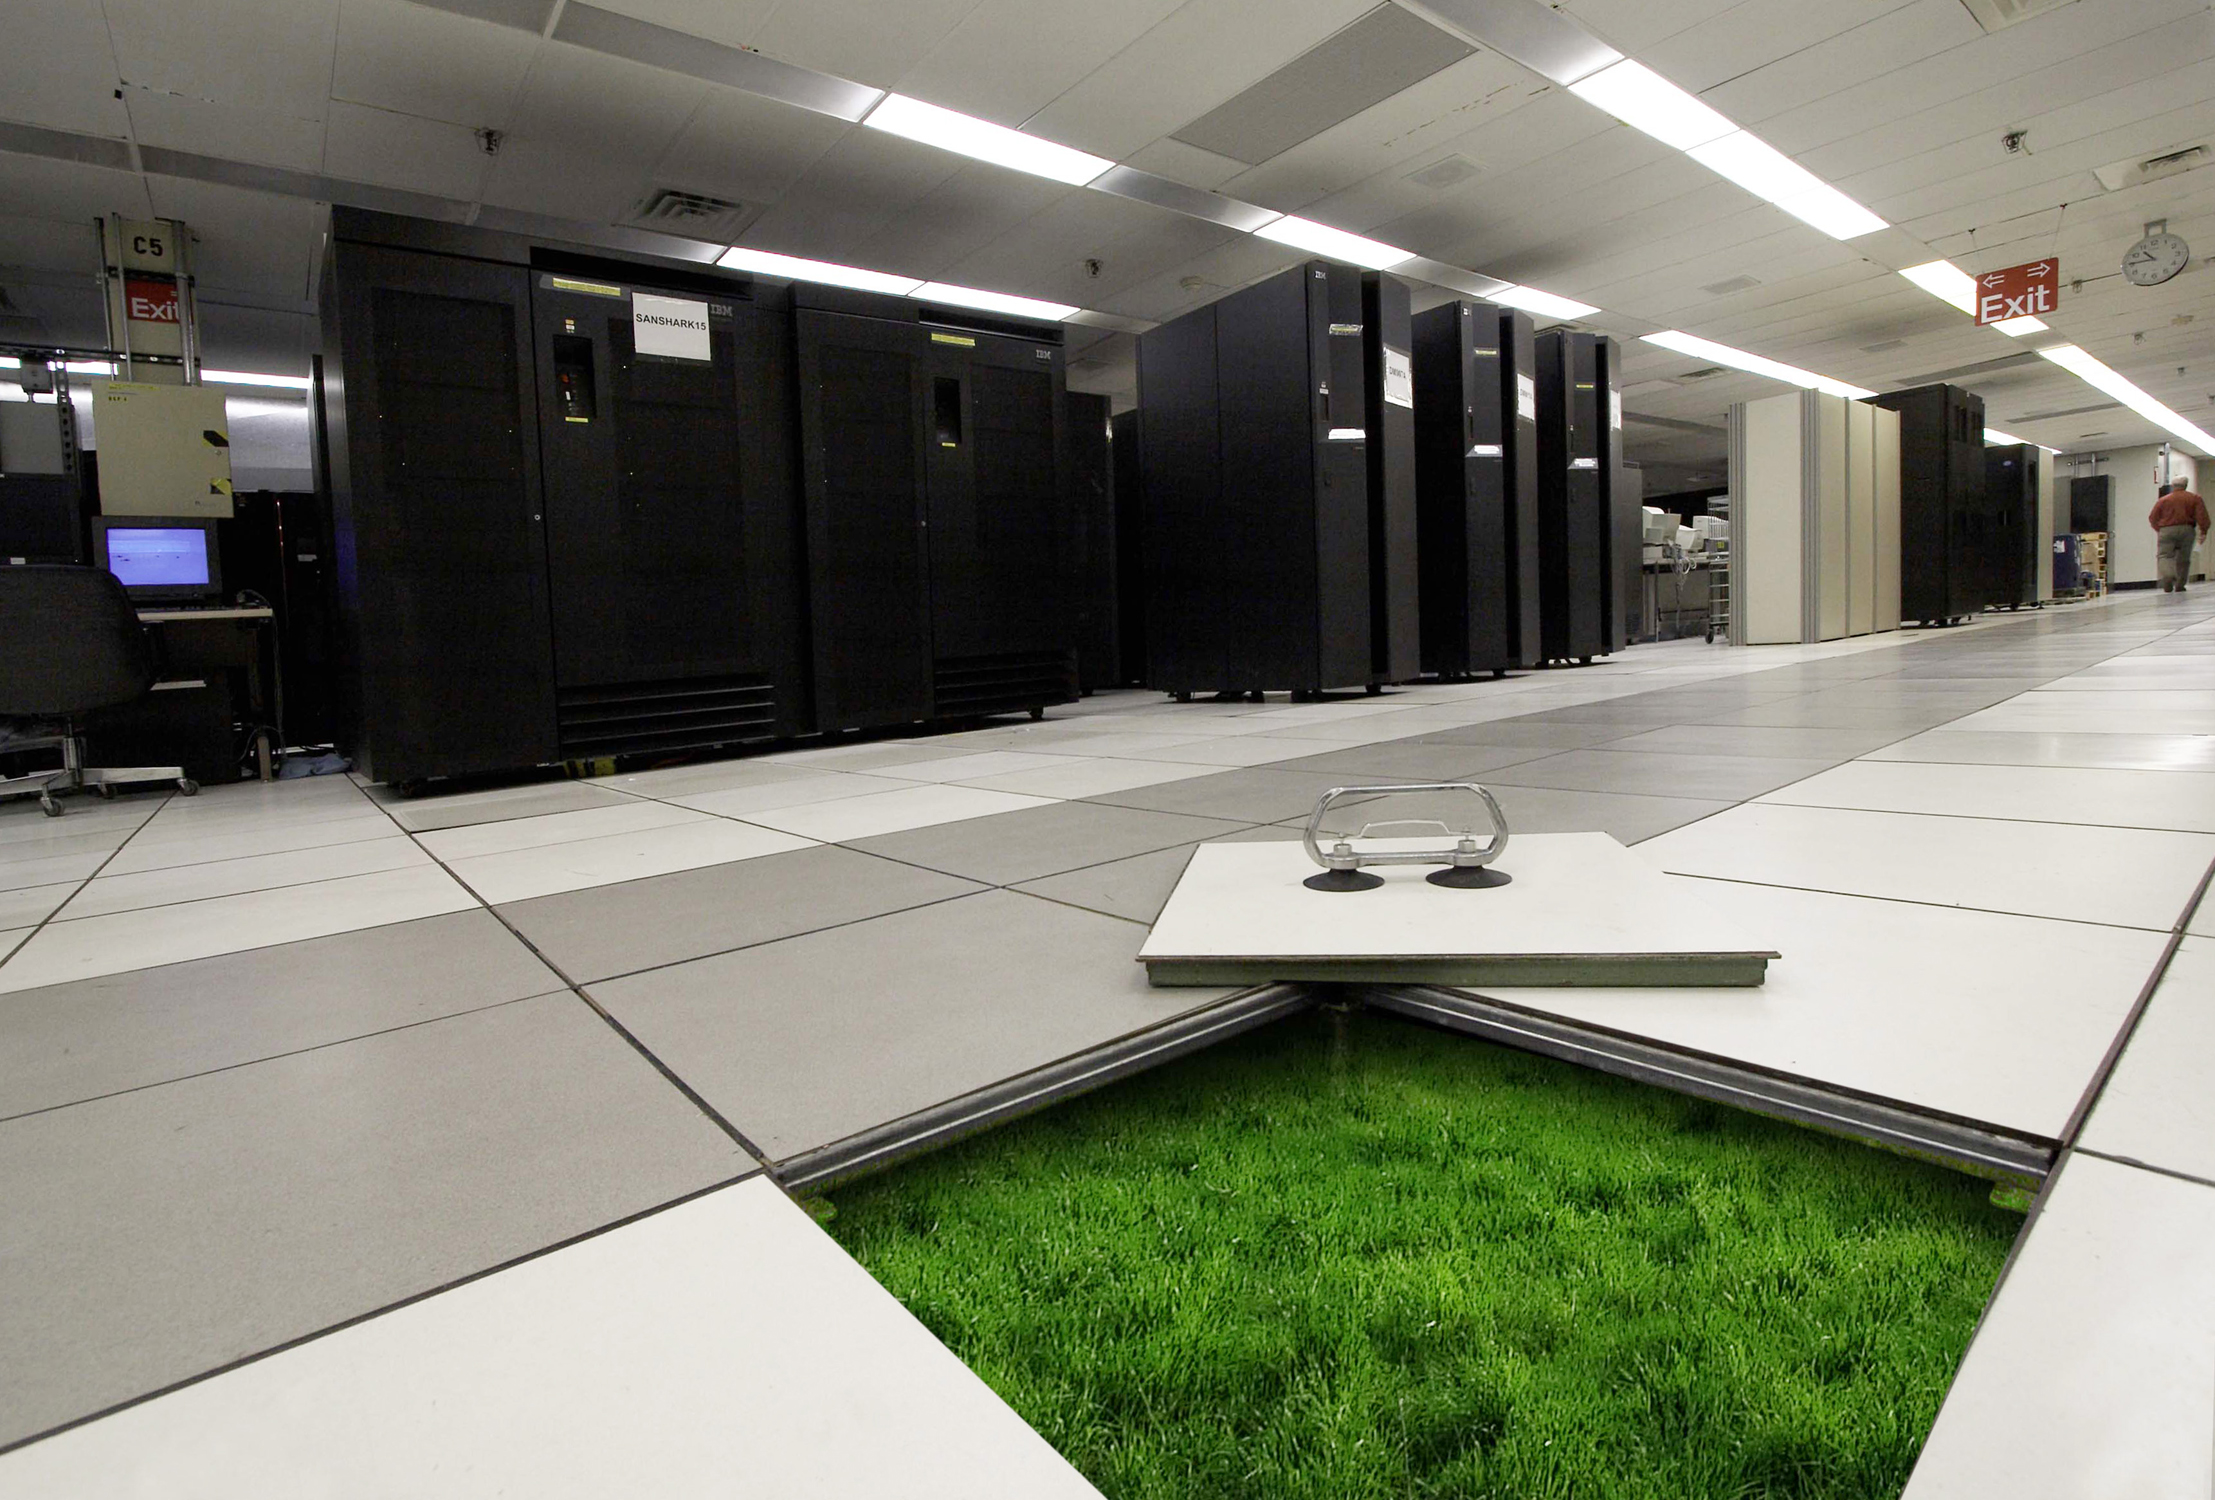
\includegraphics[width=\textwidth]{fig3}
	\caption{Diagrama do Rack}
	\label{fig3}
\end{figure}

\subsection{Topologia}
Com base na figura 2, aprenseta-se o cabeamento horizontal que interligará os wallplates até o patch panel, sendo que a maioria dos pontos terá um cabo e outros passarão 2 cabos. Será utilizado um rack de piso 42U, foi escolhido este tamanho de rack já prevendo futuras expansões tanto de cabeamento quanto de instalação de servidores e outros equipamentos no rack. Com base na figura 3, podemos observar o patch panel 2U de 48 portas na parte superior do rack, o qual interligará com patch cords no switch. Mais abaixo no rack serão instalados os equipamentos de link de internet e vlan de fibra óptica. 


\subsection{Encaminhamento}
Os cabos serão lançados por meio dos eletrodutos corrugados já instalados nas paredes que levam diretamente a ER (Equipament Room). Os eletrodutos são da marca Tigre e cor amarela e são do tamanho de 3/4". Para maioria dos pontos será lançado apenas 1 cabo, sendo que os pontos que precisam de impressoras ao lado dos computadores comportarão 2 cabos. Os cabos serão lançados por meio de guia para facilitar o lançamento. 

\subsection{Memorial descritivo}
Para toda esta instalação de cabeamento estruturado foi realizado um processo licitatório do tipo Pregão Presencial realizado pela Prefeitura Municipal. Segue abaixo quantidade e descrição dos itens:
\begin{itemize}
\item 01	Switch Gigabit 1U 48+4 portas SFP HP Aruba 1920S;
\item 01	Patch Panel 2U 48 portas Fugukawa Gigalan Cat6;
\item 50	Patch Cords 1,5m Fugukawa Gigalan Cat6 cor amarela;
\item 20	Patch Cords 3m Fugukawa Gigalan Cat6 cor azul;
\item 20	Patch Cords 5m Fugukawa Gigalan Cat6 cor vermelha;
\item 50	Conectores RJ45 fêmea Fugukawa Gigalan Cat6;
\item 30 	Espelhos 1 posição Fugukawa;
\item 10 	Espelhos 2 posição Fugukawa;
\item 02	Caixas (305m cada) de cabo de rede UTP Fugukawa Gigalan Cat6 cor vermelha;
\item 01 	Rack fechado de piso 42U IPMETAL (800mm) já com 2 bandejas; guias verticais; 2 guias horizontais e uma régua com 12 tomadas 10A;
\item 01	Nobreak de Rack 2U 1200VA NHS Compact Plus. 
\end{itemize}

\subsection{Identificação dos cabos}
O cabeamento estruturado será identificado de forma bem simples, para os pontos das áreas de trabalho serão etiquetados com nomenclatura PT01; PT02 por diante. Estes mesmo serão identificados no Patch Panel desta mesma forma. Já a identificação dos Patch cords entre o Patch Panel e o Switch terão a nomenclatura SW01; SW02 em diante. O patch cord que conectará o link de internet ao Switch terá a nomenclatura de LNK1. 

\section{Implantação}
O cronograma de implantação será, respectivamente, a montagem do rack, instalação dos cabos e identificação dos cabos.
Todo o cabeamento; conectores; wallplates; patch cords e patech panel serão da marca Furukawa Gigalan padrão cat6. O rack e demais acessórios do rack (guias verticais; bandejas fixas; guias de cabo; régua de tomadas) serão da marca IpMetal e o Switch será um HPE Aruba 1920S 48 + 4SFP. Os colaboradores responsáveis pela instalação e montagem optaram pela instalação do padrão EIA/TIA 568A para o cabeamento e terão um cronograma de 3 dias para realizar todo o trabalho. Estes dias serão definidos entre a equipe e o Secretário de Saúde.

\section{Plano de certificação}
O projeto não contará com plano de certificação pois como se trata de um órgão público, o orçamento não prevê esse tipo de situação e também a falta de conhecimento do assunto por parte dos superiores se torna um empecilho. Talvez no futuro tendo uma real necessidade de certificar a rede, a Prefeitura poderá realizar uma licitação para que uma empresa terceirizada realize a certificação ou até mesmo licite os equipamentos de certificação para que os próprios colaboradores do Departamento de Tecnologias e Sistemas de Informação realizem a certificação da rede não somente neste prédio, como também em todas as demais redes existentes na Prefeitura. 

\section{Plano de manutenção}
As revisões na rede acontecerão com visitas periódicas ao local e com o frequente monitoramento via softwares no datacenter principal.

\subsection{Plano de expansão}
Existe hoje um plano de expansão, foram instalados 15 pontos a mais e estratégicos de rede, deste modo, a rede já está pronta para expandir para um número máximo de 41 pontos de rede, pois serão utilizados até 7 pontos de rede para interconectar outros dispositivos na sala do rack. Fechando assim 48 conexões máximas possíveis no switch que será instalado. Caso no futuro haja a necessidade de mais pontos de rede, será necessário comprar cabo; conectores; switch e demais equimantos para devida expansão.

%%\section{Risco}
%%Enumerar e explicar os riscos do projeto.

%%\section{Orçamento}
%%Crie uma relação de orçamentos baseado na seções anteriores.

%%\section{Recomendações}
%%Observações e recomendações para o cliente.

\section{Referências bibliográficas}
%%Utilize o mendley, o jabref ou diretamente o bibtex para gerenciar suas referências biliográficas. %%As referências são criadas automaticamente de acordo com o uso no texto.
%%Exemplo: Redes de computadores, segundo \cite{t2013} é considerada..... Já \cite{kurose2010} %%apresenta uma versão...
%%Analisando os pressupostos de \cite{ref3} e \cite{ref4} concluimos que....
\renewcommand\refname{} %%Referências bibliográficas}  
\bibliographystyle{ieeetr}
\bibliography{referencias}  

%% ***********************************************************************

\end{document}